\documentclass[a4paper,12pt]{report}
\usepackage{import}
\usepackage{graphicx}
\usepackage{amsmath}
\usepackage[utf8]{inputenc}
\usepackage{mathptmx}
\usepackage{physics}
\usepackage{multicol}
\usepackage{listings}
\usepackage{color}
\usepackage{acro}
\usepackage{filecontents}
\usepackage[noadjust]{cite}
\usepackage{titlesec}

\titlespacing*{\chapter}{0pt}{0pt}{0pt}
\renewcommand{\baselinestretch}{1.5}
\setlength{\columnsep}{1cm}
\usepackage[%
    left=1.0in,%
    right=1.0in,%
    top=1.0in,%
    bottom=1.0in,%
]{geometry}%
\begin{document}
\import{section/}{cover.tex}
\import{section/}{supervisor-ecommendation.tex}
\import{section/}{approval.tex}

\pagenumbering{roman}
\setcounter{page}{1}
\import{section/}{abstract.tex}   
\import{section/}{abbreviation.tex}  

       
\tableofcontents

 
\thispagestyle{empty} 
\listoffigures 
\newpage

\clearpage
\setcounter{page}{1}
\pagenumbering{arabic}

\chapter{Introduction}
\section{Background}
Artificial neural network (ANN), usually called Neural Network (NN), is an
algorithm that was originally motivated by the goal of having machines that
can mimic the brain. A neural network consists of an interconnected group of
artificial neurons. They are physical cellular systems capable of obtaining,
storing information, and using experiential knowledge. Like human brain, the
ANN’s knowledge comes from examples that they encounter. In human
neural system, learning process includes the modifications to the synaptic
connections between the neurons. In a similar way, ANNs adjust their
structure based on output and input information that flows through the
network during the learning phase.
00
Data processing procedure in any typical neural network has two major steps:
the learning and application step. At the first step, a training database or
historical price data is needed to train the networks. This dataset includes an
input vector and a known output vector. Each one of the inputs and outputs
are representing a node or neuron. In addition, there are one or more hidden
layers. The objective of the learning phase is to adjust the weights of the
connections between different layers or nodes. After setting up the learning
samples, in an iterative approach a sample will be fed into the network and
Artificial Neural Network.

\section{Problem statement}
Logic gates are the fundamental components to build any digital system. The devices we encounter in our daily life is using them for certain. Logic gates has been using as a base example to understand the ANN. Though logic gates example has no practical use in the field of AI, but it gives fundamental concept about single and multilayer perceptron. Logic gates can be divided into three categories for ANN problem, i. Single input linearly separable eg. NOT ii. Double input linearly separable eg. OR, AND etc. iii. Linearly not separable eg. XOR. The linearly separable gates can be implemented using single perceptron whereas linearly non separable gates cannot  implement using single perceptron. The concept of back-propagation is used to solved linearly non separable problem. 

\section{Objective}
Implementing a logic gates in ANN is a general problem in the field of artificial intelligence. The main objective of this report is to understand the fundamental concept of artificial intelligence, and how does a machine can mimic a human brain. Understand the mathematics behind single and multilayer perceptron network is another objective of this report. Implementation of logic gates into our perceptron model is the final objective of this report.


\section{Limitations of report}
Limitation of this report are:
\begin{itemize}
	\item This report is more about informative rather than a research.
\end{itemize}

\chapter{LITERATURE REVIEW}
\section{Previous Works, Discussions and Findings}
The history of Artificial Intelligence (AI) began in antiquity, with myths, stories and rumors of artificial beings endowed with intelligence or consciousness by master craftsmen. The seeds of modern AI were planted by classical philosophers who attempted to describe the process of human thinking as the mechanical manipulation of symbols. This work culminated in the invention of the programmable digital computer in the 1940s, a machine based on the abstract essence of mathematical reasoning. In the 1940s and 50s, a handful of scientists from a variety of fields (mathematics, psychology, engineering, economics and political science) began to discuss the possibility of creating an artificial brain. The field of artificial intelligence research was founded as an academic discipline in 1956.

In 1950 Alan Turing published a landmark paper in which he speculated about the possibility of creating machines that think\cite{5}. He noted that "thinking" is difficult to define and devised his famous Turing Test. If a machine could carry on a conversation (over a teleprinter) that was indistinguishable from a conversation with a human being, then it was reasonable to say that the machine was "thinking". This simplified version of the problem allowed Turing to argue convincingly that a "thinking machine" was at least plausible and the paper answered all the most common objections to the proposition. The Turing Test was the first serious proposal in the philosophy of artificial intelligence. In 1951, using the Ferranti Mark 1 machine of the University of Manchester, Christopher Strachey wrote a checkers program and Dietrich Prinz wrote one for chess. Arthur Samuel's checkers program, developed in the middle 50s and early 60s, eventually achieved sufficient skill to challenge a respectable amateur. Game AI would continue to be used as a measure of progress in AI throughout its history.

The Dartmouth Conference of 1956 was organized by Marvin Minsky, John McCarthy and two senior scientists: Claude Shannon and Nathan Rochester of IBM. The proposal for the conference included this assertion: "every aspect of learning or any other feature of intelligence can be so precisely described that a machine can be made to simulate it". The participants included Ray Solomonoff, Oliver Selfridge, Trenchard More, Arthur Samuel, Allen Newell and Herbert A. Simon, all of whom would create important programs during the first decades of AI research. At the conference Newell and Simon debuted the "Logic Theorist" and McCarthy persuaded the attendees to accept "Artificial Intelligence" as the name of the field. The 1956 Dartmouth conference was the moment that AI gained its name, its mission, its first success and its major players, and is widely considered the birth of AI. The term "Artificial Intelligence" was chosen by McCarthy to avoid associations with cybernetics and connections with the influential cyberneticist Norbert Wiener. The years after the Dartmouth conference were an era of discovery, of sprinting across new ground. The programs that were developed during this time were, to most people, simply "astonishing": computers were solving algebra word problems, proving theorems in geometry and learning to speak English. Few at the time would have believed that such "intelligent" behavior by machines was possible at all. Researchers expressed an intense optimism in private and in print, predicting that a fully intelligent machine would be built in less than 20 years. Government agencies like DARPA poured money into the new field.

In the 1970s, AI was subject to critiques and financial setbacks. AI researchers had failed to appreciate the difficulty of the problems they faced. Their tremendous optimism had raised expectations impossibly high, and when the promised results failed to materialize, funding for AI disappeared. At the same time, the field of connectionism (or neural nets) was shut down almost completely for 10 years by Marvin Minsky's devastating criticism of perceptrons. Despite the difficulties with public perception of AI in the late 70s, new ideas were explored in logic programming, commonsense reasoning and many other areas.

The perceptron algorithm was invented in 1958 at the Cornell Aeronautical Laboratory by Frank Rosenblatt, funded by the United States Office of Naval Research.The perceptron was intended to be a machine, rather than a program, and while its first implementation was in software for the IBM 704, it was subsequently implemented in custom-built hardware as the "Mark 1 perceptron". This machine was designed for image recognition: it had an array of 400 photocells, randomly connected to the "neurons". Weights were encoded in potentiometers, and weight updates during learning were performed by electric motors.

Although the perceptron initially seemed promising, it was quickly proved that perceptrons could not be trained to recognise many classes of patterns. This caused the field of neural network research to stagnate for many years, before it was recognised that a feedforward neural network with two or more layers (also called a multilayer perceptron) had far greater processing power than perceptrons with one layer (also called a single layer perceptron).Single layer perceptrons are only capable of learning linearly separable patterns; in 1969 a famous book entitled Perceptrons by Marvin Minsky and Seymour Papert showed that it was impossible for these classes of network to learn an XOR function. It is often believed (incorrectly) that they also conjectured that a similar result would hold for a multi-layer perceptron network. However, this is not true, as both Minsky and Papert already knew that multi-layer perceptrons were capable of producing an XOR function.Nevertheless, the often-miscited Minsky/Papert text caused a significant decline in interest and funding of neural network research. It took ten more years until neural network research experienced a resurgence in the 1980s. This text was reprinted in 1987 as "Perceptrons - Expanded Edition" where some errors in the original text are shown and corrected.
\subsection{Backpropagation}
Its modern version (also called the reverse mode of automatic differentiation) was first published in 1970 by Finnish master student Seppo Linnainmaa.

The minimization of errors through gradient descent (Cauchy 1847, Hadamard, 1908) in the parameter space of complex, nonlinear, differentiable, multi-stage, NN-related systems has been discussed at least since the early 1960s (e.g., Kelley, 1960; Bryson, 1961; Bryson and Denham, 1961; Pontryagin et al., 1961; Dreyfus, 1962; Wilkinson, 1965; Amari, 1967; Bryson and Ho, 1969; Director and Rohrer, 1969), initially within the framework of Euler-LaGrange equations in the Calculus of Variations (e.g., Euler, 1744).

Steepest descent in the weight space of such systems can be performed (Bryson, 1961; Kelley, 1960; Bryson and Ho, 1969) by iterating the chain rule (Leibniz, 1676; L'Hopital, 1696) à la Dynamic Programming (DP, Bellman, 1957). A simplified derivation of this back-propagation method uses the chain rule only (Dreyfus, 1962).

The systems of the 1960s were already efficient in the DP sense. However, they backpropagated derivative information through standard Jacobian matrix calculations from one "layer" to the previous one, without explicitly addressing either direct links across several layers or potential additional efficiency gains due to network sparsity (but perhaps such enhancements seemed obvious to the authors).

Explicit, efficient error backpropagation (BP) in arbitrary, discrete, possibly sparsely connected, NN-like networks apparently was first described in a 1970 master's thesis (Linnainmaa, 1970, 1976), albeit without reference to NNs. BP is also known as the reverse mode of automatic differentiation (e.g., Griewank, 2012), where the costs of forward activation spreading essentially equal the costs of backward derivative calculation. See early BP FORTRAN code (Linnainmaa, 1970) and closely related work (Ostrovskii et al., 1971).

BP was soon explicitly used to minimize cost functions by adapting control parameters (weights) (Dreyfus, 1973). This was followed by some preliminary, NN-specific discussion (Werbos, 1974, section 5.5.1), and a computer program for automatically deriving and implementing BP for any given differentiable system (Speelpenning, 1980).

To my knowledge, the first NN-specific application of efficient BP as above was described by Werbos (1982). Related work was published several years later (Parker, 1985; LeCun, 1985). When computers had become 10,000 times faster per Dollar and much more accessible than those of 1960-1970, a paper of 1986 significantly contributed to the popularisation of BP for NNs (Rumelhart et al., 1986), experimentally demonstrating the emergence of useful internal representations in hidden layers.

Compare also the first adaptive, deep, multilayer perceptrons (the GMDH networks; Ivakhnenko et al., since 1965), whose layers are incrementally grown and trained by regression analysis, as well as a more recent method for multilayer threshold NNs (Bobrowski, 1978).

\chapter{METHODOLOGY}
\section{Perceptron}
Perceptrons were developed in the 1950s and 1960s by the scientist Frank Rosenblatt, inspired by earlier work by Warren McCulloch and Walter Pitts.
Perceptron can be defined as an algorithm for learning a binary classifier called a threshold function: a function that maps its input 
$x$ (a real-valued vector) to an output value $f(x)$ (a single binary value):
\begin{equation}
f(x)=
\begin{cases}
    1,& \text{if } w*x+b > 1\\
    0,              & \text{otherwise}
\end{cases}
\end{equation}

where w  is a vector of real-valued weights, w.x is the dot product $\sum_{i=1}^m w_i x_i$ where m is the number of inputs to the perceptron, and b is the bias. The bias shifts the decision boundary away from the origin and does not depend on any input value.

\begin{figure}[htp]
\centering
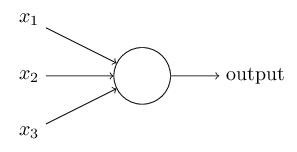
\includegraphics[scale=0.300]{resources/image-01.png}
\caption{Single layer perceptron}
\label{}
\end{figure}

In the example shown the perceptron has three inputs, $x_1,x_2,x_3$. In general it could have more or fewer inputs. Rosenblatt proposed a simple rule to compute the output. He introduced weights, $w_1,w_2,…$, real numbers expressing the importance of the respective inputs to the output. The neuron's output, 0 or 1, is determined by whether the weighted sum is less than or greater than some threshold value. Just like the weights, the threshold is a real number which is a parameter of the neuron. To put it in more precise algebraic terms:
\begin{equation}
f(x)=
\begin{cases}
    0,& \text{if } \sum_j{w_j x_i} \leq \text{Threshold}\\
    1, & \text{if }  \sum_j{w_j x_i} > \text{Threshold}
\end{cases}
\end{equation}

The condition threshold is cumbersome, and we can make two notational changes to simplify it. The first change is to write $\sum_j{w_j x_i}$ as a dot product, $w.x=\sum_j{w_j x_i}$ , where w and x are vectors whose components are the weights and inputs, respectively. The second change is to move the threshold to the other side of the inequality, and to replace it by what's known as the perceptron's bias, $b=- \text{Threshold}$  Using the bias instead of the threshold, the perceptron rule can be rewritten:

\begin{equation}
f(x)=
\begin{cases}
    1,& \text{if } w*x+b > 1\\
    0,              & \text{otherwise}
\end{cases}
\end{equation}

\section{Learning Rule}
We defined the algorithm for a single perceptron unit. Let’s consider a ex-
ample for OR gate. OR gate has two inputs and one output, it gives output
1 when atleast one of it’s input is 1, otherwise 0. Let’s Draw a perceptron
to mimic OR gate as follows.
\begin{figure}[htp]
\centering
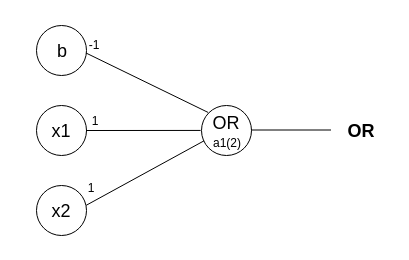
\includegraphics[scale=0.4]{resources/image-02.png}
\caption{OR gate perceptron unit}
\label{}
\end{figure}

\begin{table}
\centering
\begin{tabular}{|l|c|c|l|}
	$x_1$ & $x_2$ & $\sum_j{w_j x_i}$ & $y$ \\
	0 & 0 & -1 & 0\\
	0 & 1 & 0 & 1\\
	1 & 0 & 0 & 1\\
	1 & 1 & 1 & 1\\
\end{tabular}
\end{table}
In the above example, x 1 , x 2 are two inputs for perceptron which is to
mimic the two inputs of OR gate, b is defined as bais, -1, 1 and 1 are the
weights for bais and two inputs.
Here, we defined weight as hit and trail basis, we require some rule so
that, perceptron itself update their weight to satisfy given condition.
\subsection{Perceptron Learning Rule}
This rule is an error correcting the supervised learning algorithm of single layer feedforward networks with linear activation function, introduced by Rosenblatt.

 As being supervised in nature, to calculate the error, there would be a comparison between the desired/target output and the actual output. If there is any difference found, then a change must be made to the weights of connection.
 
 To explain its mathematical formulation, suppose we have ‘n’ number of finite input vectors, $x_n$, along with its desired/target output vector $t_n$, where n = 1 to N.

Now the output ‘y’ can be calculated, as explained earlier on the basis of the net input, and activation function being applied over that net input can be expressed as follows 
\begin{equation}
f(x)=
\begin{cases}
    0,& \text{if } \sum_j{w_j x_i} \leq \text{Threshold}\\
    1, & \text{if }  \sum_j{w_j x_i} > \text{Threshold}
\end{cases}
\end{equation}
The updating of weight can be done in the following two cases:

Case I:  when $t \neq y$, then
\begin{equation}
w_i=w_i +\Delta w_i 
\end{equation}
Where,
\begin{equation}
\Delta w_i = \eta (t - y) w_i 
\end{equation}
\begin{equation}
y = (\sum_j{w_j x_i} \geq 0)
\end{equation}
\begin{equation}
\eta = Learning rate
\end{equation}
Case II: when t = y, then,
No change in weight.
\subsection{Gradient Descent/Delta Rule}
The Delta Rule, [also known as the Widrow \& Hoff Learning rule or the Least Mean Square (LMS) rule] was invented by Widrow and Hoff in early 1960s. This rule is similar to the perceptron learning rule by McClelland \& Rumelhart, 1988, but is also characterized by a mathematical utility and elegance missing in the perceptron and other early learning rules. Delta rule tries to minimize the error between target value and output value measured by error function also known as cost function. The Delta Rule employs the error function for what is known as Gradient Descent learning, which involves the ‘modification of weights along the most direct path in weight-space to minimize error’, so change applied to a given weight is proportional to the negative of the derivative of the error with respect to that weight. The Error/Cost function is commonly given as the sum of the squares of the differences between all target and actual node activation for the output layer. For a particular training pattern (i.e., training case), error is thus given by:

\begin{equation}
a=\sum_i {x_i w_i}
\end{equation}
\begin{equation}
E(p)=1/2 \sum_i {}(t-a)^2
\end{equation}
where, E(p) is error over an entire set of training patterns (i.e., over one iteration, or epoch). Total Error is given by
\begin{equation}
E=1/2 \sum_p \sum_i{}(t-a)^2
\end{equation}
 Calculate the derivative (gradient) of the Cost Function with respect
to the weights, and then change each weight by a small increment in
the negative (opposite) direction to the gradient,
\begin{equation}
\dv{E(p)}{w_i}=(t-a)(-x_i)
\end{equation}


\begin{figure}[htp]
\centering
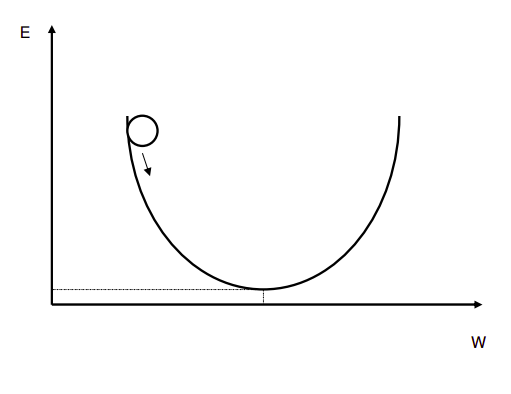
\includegraphics[scale=.40]{resources/image-03.png}
\caption{Graphical Representation of Gradient Descent}
\label{}
\end{figure}
To reduce E by gradient descent, move/increment weights in the
negative direction to the gradient,


Gradient descent Learning rule is given by
\begin{equation}
W = W(old)+ \Delta W
\end{equation}
\begin{equation}
\Delta W = \eta (t-a)(-x_i)
\end{equation}


\section{MultiLayer Perceptron}
Rosenblatt purposed the perceptron as the first model for learning with a teacher(i.e. supervised learning) in 1958. Later, it came to know that the perceptron couldn't solve even XOR problem. The perceptron purposed by Rosenblatt could only solve lineary separable problem, but most of the real world problem are lineary non separable problem, which stagnated the reasearch in artificial intellegence fields to next decade. The first remarkable learning algorithm to solve the limitation of perceptron problem was introduced in 1986, in the paper titled "Learning representations back-propagating errors". Let's us consider one input, one hidden and one output layer as shown in figure:
\begin{figure}[htp]
\centering
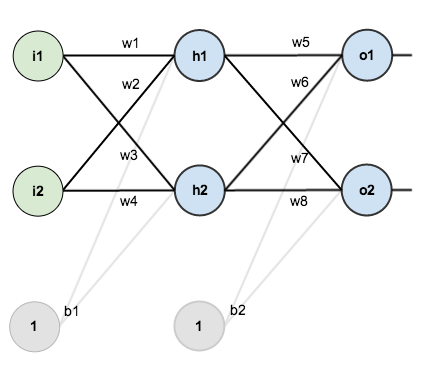
\includegraphics[scale=0.5]{resources/image-06.png}
\caption{Multilayer perceptron Network}
\label{}
\end{figure} 

In the above figure, $i_1$ \& $i_2$ are two inputs to the neural network, $h_1$ \& $h_2$ are hidden layer and $o_1$ and $o_1$ are two output layer nodes.
Multilayer perceptron works in two steps, at first it goes in forward direction to get output same as perceptron rule which is called feedforward neural network. The second steps is it iterates backward one layer at a time to update the weights to minimize the loss. The backpropagation algorithm works by computing the gradient of the loss function with respect to each weight by the chain rule.

In feedforward network,

\begin{equation}
h_1 = i_1 * w_1 + i_2 * w_2+ b_1
\end{equation},
Output at other nodes is also given by,
\begin{equation}
h_2 = i_1 * w_3 + i_4 * w_2+ b_1
\end{equation}
\begin{equation}
o_1 = h_1 * w_5 + h_2 * w_6+ b_2
\end{equation}
\begin{equation}
o_2 = h_1 * w_7 + h_2 * w_8+ b_2
\end{equation}
And each node output goes to the next layer passes through sigmoid activation function. for example,
output at $o_1$ is given by,
\begin{equation}
Out_{o1} = \frac{1}{1+e^{-o_1}} 
\end{equation}

\subsubsection*{Backpropagation},
Backpropagation updates the weigths iteratively in backwards direction one layer at a time from the last layer to mimizes the error. Error can be simply written as the difference between the predicted outcome and the actual outcome. Mathematically:
\begin{equation}
Error = \sum (t-o)
\end{equation}
where t is target/expected outcome \& o is predicted outcome.


However, Error can be both negative and positive, which may cancel out each other and produces no error, to solve this problem, gradient descent uses square of error.  Further, this error is divided by 2, to make it easier to differentiate.
Then total error is given by,
\begin{equation}
E_{total} = \frac{1}{2} \sum (t_1-o_1)^2 + (t_2-o_2)^2
\end{equation}
Since, there may be many weights contributing to this error, we take the partial derivative, to find the minimum error, with respect to each weight at a time. Error at output layer $w_5$ is given by

\begin{equation}
\frac{\partial E_{total}}{\partial w_5} = \frac{\partial E_{total}}{\partial Out{o_1}} * \frac{\partial Out_{o_1}}{\partial o_1}  * \frac{\partial o_1}{\partial w_5} 
\end{equation}

From calculation,

\begin{equation}
\frac{\partial E_{total}}{\partial Out{o_1}}= - (t_1 - Out_{o1})
\end{equation}
and,
\begin{equation}
\frac{\partial Out_{o_1}}{\partial o_1}= Out_{o1} * (1 - Out_{o1})
\end{equation}
\begin{equation}
\frac{\partial o_1}{\partial w_5} = Out_{h_1}
\end{equation}
So,
\begin{equation}
\frac{\partial E_{total}}{\partial w_5} = - (t_1 - Out_{o1}) * Out_{o1} * (1 - Out_{o1}) * Out_{h_1}
\end{equation}
Updating $w_5$,
\begin{equation}
w_5 = w_5 - \eta * \frac{\partial E_{total}}{\partial w_5}
\end{equation}
and for $w_6$
\begin{equation}
w_6 = w_6 - \eta * \frac{\partial E_{total}}{\partial w_6}
\end{equation}

Similarly we can update all the weights for output layer. To update the weights for input layer, i.e $w_1$, $w_2$, $w_3$, $w_4$, let's take $w_1$ as representative,

\begin{equation}
\frac{\partial E_{total}}{\partial w_1} = \frac{\partial E_{total}}{\partial Out{h_1}} * \frac{\partial Out_{h_1}}{\partial h_1}  * \frac{\partial h_1}{\partial w_1} 
\end{equation}
and,
\begin{equation*}
\frac{\partial E_{total}}{\partial Out{h_1}} = \frac{\partial E_{1}}{\partial Out{h_1}} + \frac{\partial E_{2}}{\partial Out{h_2}}
\end{equation*}
\begin{equation}
\frac{\partial E_{total}}{\partial Out{h_1}} = \frac{\partial E_{1}}{\partial Out{o_1}} *  \frac{\partial Out_{o_1}}{\partial o_1} * \frac{\partial {o_1}}{\partial Out{h_1}}+  \frac{\partial E_{2}}{\partial Out{h_2}}
\end{equation}
\begin{equation}
\frac{\partial Out_{h_1}}{\partial h_1}= Out_{h1} * (1 - Out_{h1})
\end{equation}
\begin{equation}
\frac{\partial h_1}{\partial w_1} = i_1
\end{equation}
So,
\begin{equation}
\frac{\partial E_{total}}{\partial w_1}= ( \frac{\partial E_{1}}{\partial Out{o_1}} *  \frac{\partial Out_{o_1}}{\partial o_1} * \frac{\partial o_{1}}{\partial Out{h_1}}+  \frac{\partial E_{2}}{\partial Out{h_1}}) * (Out_{h1} * (1 - Out_{h1}))* i_1
\end{equation}

Updating $W_1$,
\begin{equation}
w_1 = w_1 -  \eta \frac{\partial E_{total}}{\partial w_1}
\end{equation},
Similary we can update the other weight i.e $w_2$, $w_3$, $w_4$ as well.



\chapter{IMPLEMENTATION, RESULT AND ANALYSIS}
Three types of implementation has been done to prove the concept of logic gates in ANN. The first one is single input Perceptron, i.e NOT gate. Perceptron implementation in python code goes here,
\lstinputlisting[language=Python,breaklines=true,tabsize=2]{code/Perceptron.py}

In the above class, we can pass no of inputs no as constructor so that we could build all types of logic gates. We train the NOT gate as follows

\begin{lstlisting}[language=Python]
import numpy as np
import matplotlib.pyplot as plt
from Perceptron import Perceptron

training_inputs = []
training_inputs.append(np.array([0]))
training_inputs.append(np.array([1]))

labels = np.array([1, 0])

perceptron = Perceptron(1)
perceptron.train(training_inputs, labels)
\end{lstlisting}

Prediction was carried out by calling the function named `predict`
\begin{lstlisting}[language=Python,breaklines=true]
inputs = np.array([0])
print("inputs"+str(inputs)+"Output"+str(perceptron.predict(inputs)))
# output => 1
inputs = np.array([1])
print("inputs"+str(inputs)+"Output"+str(perceptron.predict(inputs))) 
# output => 1
\end{lstlisting}
Prediction results the expected output, the weights during the convergence was observed -0.01 \& 0.01.
\begin{figure}[htp]
\centering
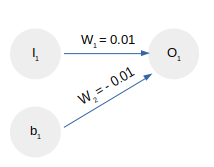
\includegraphics[scale=0.80]{resources/image-08.png}
\caption{NOT gate implementation with single perceptron}
\label{}
\end{figure}
Error vs Ephos graph is displayed as,
\begin{figure}[htp]
\centering
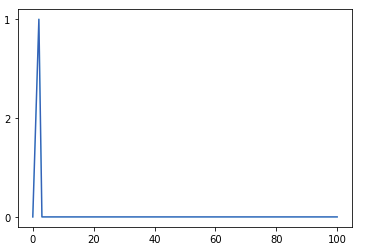
\includegraphics[scale=0.80]{resources/image-07.png}
\caption{Error during NOT gate convergence}
\label{}
\end{figure}

\subsubsection*{AND gate}
Same perceptron class can be used to train AND or OR gate. Training a AND gate can be done as

\subsubsection*{Prepare the datasets}
\begin{lstlisting}[language=Python]
training_inputs = []
training_inputs.append(np.array([1, 1]))
training_inputs.append(np.array([1, 0]))
training_inputs.append(np.array([0, 1]))
training_inputs.append(np.array([0, 0]))

labels = np.array([1, 0, 0, 0])
\end{lstlisting}


\subsubsection*{Train the model}
\begin{lstlisting}[language=Python]
perceptron = Perceptron(2)
perceptron.train(training_inputs, labels)
\end{lstlisting}
 
Here, 2 in the constructor of Perceptron class is the no of input nodes.


\subsubsection*{Test}
\begin{lstlisting}[language=python]
inputs = np.array([0, 0])
print("inputs"+str(inputs)+"Output "+str(perceptron.predict(inputs)))

inputs = np.array([0, 1])
print("inputs"+str(inputs)+"Output "+str(perceptron.predict(inputs)))

inputs = np.array([1, 0])
print("inputs"+str(inputs)+"Output "+str(perceptron.predict(inputs)))

inputs = np.array([1, 1])
print("inputs"+str(inputs)+"Output "+str(perceptron.predict(inputs)))
\end{lstlisting}
Prediction results the expected output, the weights during the convergence was observed [-0.02, 0.01,  0.02].  

\begin{figure}[htp]
	\centering
	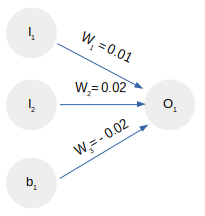
\includegraphics[scale=0.60]{resources/image-10.png}
	\caption{AND gate implementation with single perceptron}
	\label{}
\end{figure}
Error vs Ephos graph is displayed as,
\begin{figure}[htp]
	\centering
	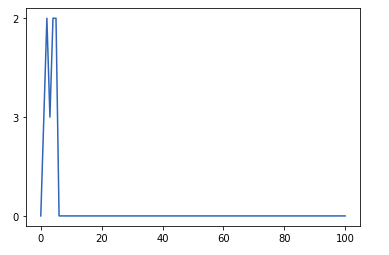
\includegraphics[scale=0.80]{resources/image-09.png}
	\caption{Error during AND gate convergence}
	\label{}
\end{figure}
\subsubsection*{XOR Gate}
Implementing a XOR gate requires multilayer perceptron network, so defined a Multilayer perceptron class.
\lstinputlisting[language=Python,breaklines=true,tabsize=2]{code/MultilayerPerceptron.py}

\subsubsection*{Prepare XOR datasets}
\begin{lstlisting}
inputs = np.array([[0,0],[0,1],[1,0],[1,1]])
labels = np.array([[0],[1],[1],[0]])
\end{lstlisting}

\subsubsection*{Train Model}
\begin{lstlisting}[language=python]
perceptron = MultilayerPerceptron(2,2,1)
perceptron.train(inputs, labels)
\end{lstlisting}


\subsubsection*{Test XOR gate}
\begin{lstlisting}
inputs = np.array([[0, 0]])
print("inputs "+str(inputs)+" Output "+str(perceptron.predict(inputs)))

inputs = np.array([[0, 1]])
print("inputs "+str(inputs)+" Output "+str(perceptron.predict(inputs)))

inputs = np.array([[1, 0]])
print("inputs "+str(inputs)+" Output "+str(perceptron.predict(inputs)))

inputs = np.array([[1, 1]])
print("inputs "+str(inputs)+" Output "+str(perceptron.predict(inputs)))
\end{lstlisting}


\subsubsection*{Results}
Prediction results the expected output, but it required almost 10,000 ephos to get converged with learning rate 0.1, We can observe the error function during the convergence as below. 

Error vs Ephos graph is displayed as,
\begin{figure}[htp]
	\centering
	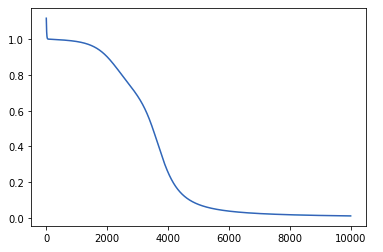
\includegraphics[scale=0.80]{resources/image-11.png}
	\caption{Error during XOR gate convergence}
	\label{}
\end{figure}



\chapter{CONCLUSION}
Depth research on single and multilayer layer perceptron is carried out, including the implmentation of idea of perceptron on logic gates. We investigated on the mathematical part of perceptron for both types of perceptron.
We explained various learning algorithm for perceptron, i.e. Perceptron Rule,gradient descent, etc. Single layer perceptron is only capable of solving linearly separable function, to overcome the defect of single layer perceptron
multilayer perceptron was introduced. Because of the limitation of single
layer perceptron reserach was stagnate for many years. 

Logic gates are divided into three categories in this report to represent all types of gates and to help analysis in ANN as well, First one is single input linearly separable. NOT gate is taken as a example of this type and implemented in Perceptron. Such types of problem can be solved with single perceptron. Second type is Double input lineary separable problem, which is also solved by single perceptron network. And last type of gates is lineary non separable gate eg. XOR gate, The concept of back propagation and multilayer perceptron has been used to solve this XOR gate problem.  


\begin{thebibliography}{}
\bibitem{1} 
Rosenblatt, Frank, “The perceptron: a probabilistic model for information storage and organization in the brain" Psychological

\bibitem{2} 
David E. Rumelhart, Geoffrey E. Hinton \& Ronald J. Williams, "Learning representations by back-propagating errors", 1986

\bibitem{3} 
Yann le cun, "A Theoretical Framework for Back-propagation"
\bibitem{4} 
Kevin Gurney, "An introduction to neural networks", 1997

\bibitem{5}
A. M. Turing, "Computing Machinery and Intelligence." Mind 49: 433-460. 1950

\bibitem{6} 
D. 0. HEBB, a Neurophysical Theory, "The Organization of Behavior", 1949
\end{thebibliography}


\end{document}
\fi